% Interaction diagram
% Author: Pascal Seppecher
% Based on diagram from Marco Miani.
\documentclass[tikz]{standalone}
\usepackage{tikz}
\usepackage{amssymb}
\usepackage{relsize}
\usetikzlibrary{positioning,matrix,decorations.pathreplacing}
\newcommand{\MonetaryLevel}{Monetary level}
\newcommand{\RealLevel}{Real level}
\newcommand{\Firms}{Firms}
\newcommand{\Households}{Households}
\newcommand{\Banks}{Banks}
\newcommand{\Commodities}{Commodities}
\newcommand{\LaborPower}{Labor power}
\newcommand{\Wages}{Wages}
\newcommand{\Consumption}{Consumption}
\newcommand{\Credits}{Credits}
\newcommand{\Withdrawals}{Withdrawals}
\newcommand{\Deposits}{Deposits}
\newcommand{\Repayments}{Repayments}
\usetikzlibrary{arrows.meta}

\newcommand{\yslant}{0.6}
\newcommand{\xslant}{-0.8}
\usetikzlibrary{calc,intersections,arrows.meta}
\usepackage{tikz-3dplot}


\colorlet{myRed}{red!20}
\tikzset{
	rows/.style 2 args={/utils/temp/.style={row ##1/.append style={nodes={#2}}},
		/utils/temp/.list={#1}},
	columns/.style 2 args={/utils/temp/.style={column ##1/.append style={nodes={#2}}},
		/utils/temp/.list={#1}}}
\makeatletter
\tikzset{anchor/.append code=\let\tikz@auto@anchor\relax,
	add font/.code=%
	\expandafter\def\expandafter\tikz@textfont\expandafter{\tikz@textfont#1},
	left delimiter/.style 2 args={append after command={\tikz@delimiter{south east}
			{south west}{every delimiter,every left delimiter,#2}{south}{north}{#1}{.}{\pgf@y}}}}
\makeatother


\tikzstyle{place}=[circle,thick,draw=blue!75,fill=blue!20,minimum size=6mm]
\tikzstyle{red place}=[place,draw=red!75,fill=red!20]
\tikzstyle{green place}=[place,draw=green!75,fill=green!20]
\tikzstyle{transition}=[rectangle,thick,draw=black!75,
fill=black!20,minimum size=4mm]


\begin{document}
	
	
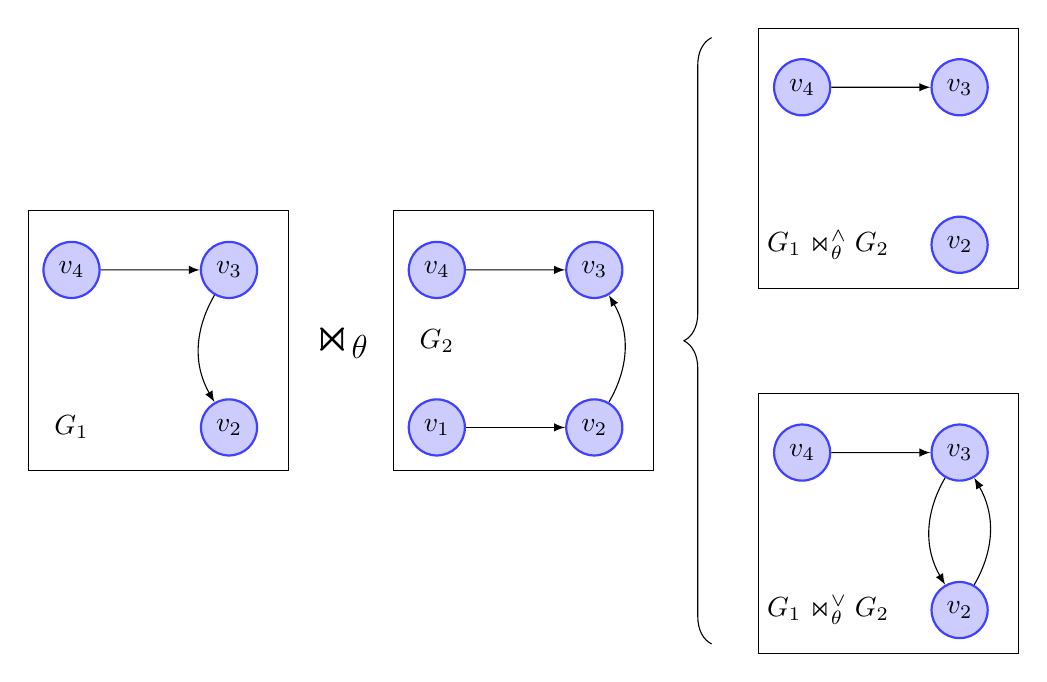
\begin{tikzpicture}[scale=1.1,on grid,
my matrix/.style={
	draw, matrix of nodes,
	nodes={
		Text Width/.expanded=\the\pgfmatrixcurrentcolumn,
		inner xsep=.1\tabcolsep, inner ysep=+0pt, align=center},
	inner sep=.1\pgflinewidth,
	font=\strut\ttfamily,
	rows={1}{fill=myRed}}
]

	\begin{scope}[
		xshift=-120,
		every node/.style={minimum size=1cm,node distance=2cm}
	]
		\draw[black, thin] (-0.5,-0.5) rectangle (2.5,2.5); 
		\node at (0,0) {$ G_1$};
		 % Agents:
		\node  (w1) {};
		\node [place] (w2) [right of=w1] {$v_2$};
		\node [place] (w3) [above of=w1] {$v_4$};
		\node [place] (w4) [above of=w2] {$v_3$};
		\draw[-latex] (w3) -- (w4);
		\draw[-latex] (w4) edge [bend right] (w2);
	\end{scope}
	
	\node (j) at (-1.1,1) {$\mathlarger{\mathlarger{\mathlarger{\mathlarger{\Join_{\theta}}}}}$};
	
		\begin{scope}[
		xshift=0,
		every node/.style={minimum size=1cm,node distance=2cm}
		]
		\draw[black, thin] (-0.5,-0.5) rectangle (2.5,2.5); 
		\node at (0,1) {$ G_2$};
		% Agents:
		\node [place] (w1) {$v_1$};
		\node [place] (w2) [right of=w1] {$v_2$};
		\node [place] (w3) [above of=w1] {$v_4$};
		\node [place] (w4) [above of=w2] {$v_3$};
		\draw[-latex] (w3) -- (w4);
		\draw[-latex] (w1) -- (w2);
		\draw[-latex] (w2) edge [bend right] (w4);
		\end{scope}
		
	
		\begin{scope}[
		xshift=120,
		yshift=60,
		every node/.style={minimum size=1cm,node distance=2cm}
		]
		\draw[black, thin] (-0.5,-0.5) rectangle (2.5,2.5); 
		\node at (0.3,0) {$ G_1\Join_\theta^\wedge G_2$};
		% Agents:
		\node  (w1) {};
		\node [place] (w2) [right of=w1] {$v_2$};
		\node [place] (w3) [above of=w1] {$v_4$};
		\node [place] (w4) [above of=w2] {$v_3$};
		\draw[-latex] (w3) -- (w4);
		\end{scope}
	
	
			\begin{scope}[
			xshift=120,
			yshift=-60,
			every node/.style={minimum size=1cm,node distance=2cm}
			]
			\draw[black, thin] (-0.5,-0.5) rectangle (2.5,2.5); 
			\node at (0.3,0) {$ G_1\Join_\theta^\vee G_2$};
			% Agents:
			\node  (w1) {};
			\node [place] (w2) [right of=w1] {$v_2$};
			\node [place] (w3) [above of=w1] {$v_4$};
			\node [place] (w4) [above of=w2] {$v_3$};
			\draw[-latex] (w2) edge [bend right] (w4);
			\draw[-latex] (w4) edge [bend right] (w2);
			\draw[-latex] (w3) -- (w4);
			\end{scope}
	 	
\draw [decorate,decoration={brace,amplitude=10pt,raise=4pt},yshift=0pt]
(3.3,-2.5) -- (3.3,4.5) node [black,midway,xshift=0.8cm] {};
	
\end{tikzpicture}
\end{document}